% указываем класс документа и стиль
\documentclass{article}
\usepackage{preamble}


\begin{document}
\selectlanguage{russian}

% == cover ==
% первую страницу не нумеруем
\thispagestyle{empty}			

\title{Оптимальный выбор группы объектов на основе анализа экспертных оценок} 
\author{Борисов К.А., Зубюк А.В.}
\maketitle

% печатаем оглавление
\tableofcontents
\newpage

\section{Экспертные оценки как субъективные суждения} 
(тут про смысл работы, актуальность. вводятся понятия субъективных суждений, экспертных оценок, приводятся требования к математическим моделям)
% 
\subsection{Принятие решений в условиях неопределённости}
\label{sec:basic_intro}

Во всех сферах человеческой деятельности информация играет роль, важность которой трудно преувеличить. В научной и деловой среде, при исследовании некоторых объектов, процессов и явлений,  предпочитают иметь дело с максимально объективной информацией о предметах исследования. Например, объективной считается информация, полученная с помощью измерительных приборов и в ходе анализа уже свершившихся фактов, если точность полученного результата достаточно высока, а сам результат можно воспроизвести в повторном исследовании. Но такая информация есть в наличии далеко не всегда.

Слово <<решение>> в русском языке имеет несколько оттенков: 
\begin{itemize}
  \item В математике решение задачи, в зависимости от её свойств, может быть найдено аналитически или численно, подобрано случайно или не совсем случайно, получено с использованием дополнительных соображений. Решение может быть или не быть единственным, а может и не существовать вовсе,  хотя во многих случаях можно переформулировать задачу так, чтобы решение всё же существовало и было единственным хотя бы с точностью до эквивалентных решений. 
  \item В более широком смысле, в практических задачах, решение часто требуется не только найти, но и {\sl принять} (иногда --- отвергнуть). Принятие такого <<волевого>> решения означает принятие человеком ответственности за его правильность решения. Человека, берущего на себя эту ответственность, будем называть {\sl лицом, принимающим решение}\footnote{Вообще говоря, лицом, принимающим решение, может быть как физическое, так и юридическое лицо, так и группа физических или юридических лиц.}. 
\end{itemize}
Например, задача выбора объектов в настоящей работе рассматривается и как проблема, требующая принятия <<волевого>> решения, и как математическая экстремальная задача. Решение экстремальной называют оптимальным, и мы используем это слово в названии настоящей работы. Но следует помнить, что найденное оптимальное решение может быть отвергнуто лицом, принимающим <<волевое>> решение.

Итак, пусть по итогам некоторого исследования требуется принять некое решение. Исследование может проводить само лицо, принимающее решение, однако в некоторых случаях требуется помощь {\sl экспертов}. Например, это происходит,  если предметы исследования не покрываются одной конкретной предметной областью, а находятся в самых разных предметных областях.  

Если отсутствует существенная для принятия решения объективная информация о предметах исследования, будем говорить о принятии решения {\sl в условиях неопределённости}. 

Объективная информация о предметах исследования, существенная для принятия решения, есть в наличие не всегда, особенно

существуют задачи, требующие принятия решения в условиях неопределённости.
--- когда одних лишь объективных данных о предмете исследования не хватает для поиска решения, оптимального в некотором смысле, и нет времени или даже принципиальной возможности их  получить. Например, можно говорить о работе в условиях неопределённости, если верны некоторые из следующих утверждений:
\begin{itemize}
 \item отсутствует фактическая информации о предмете исследования за достаточно продолжительный период времени (статистические данные);
 \item нет возможности количественного моделирования всех факторов, оказывающих существенное влияние на принятие решения, в наличии имеется только информация, отражающей качественную сторону явлений; 
 \item исследуется процесс, направление развития которого нетривиальным образом зависит от ещё не случившихся событий, которые могут случиться или не случиться в будущем;
 \item исследуется качественно новое явление или объект в процессе их развития, который уникален.
\end{itemize}

Та или иная процедура принятия решения может считаться оптимальной в практическом смысле. 
% к этому абзацу нужны ссылки на другие примеры стратегий выбора в литературе (Миша?)\

В условиях нехватки объективных данных важную роль для принятия решения играет суждение, высказанное экспертом, человеком, без строгого обоснования и твёрдой опоры на факты. Такое суждение, вообще говоря, не является объективным, поэтому будем обозначать его одним из следующих эквивалентных словосочетаний:
 \begin{itemize}
	\item субъективное суждение;
	\item субъективное мнение;
	\item экспертное мнение;
	\item ответ эксперта (на заданный ему вопрос). 
 \end{itemize}

Приглашённый эксперт может высказать суждение как \todo{В произвольной форме}самопроизвольно, так и в ответ на вопросы, специально сформулированные для поддержки принятия какого-либо решения. Процесс подготовки вопросов и прочих материалов, получения и последующего анализа экспертных мнений будем называть {\sl экспертным опросом} или {\sl экспертизой}. Лицо, принимающее решение, или субъект, от имени которого действует это лицо, выступает здесь в роли {\sl заказчика экспертизы}. От экспертов оно получает ответы на поставленные вопросы.
 
Если задача принятия решения в условиях неопределённости имеет научно-технический характер, то иногда её решение уже назревает в мозгу специалистов, работающих в соответствующей области. Однако, это решение может быть ещё не оформлено в виде мыслей, имеющих достаточную чёткость для выражения. Экспертный опрос помогает осознать и формализовать эти мысли, после чего на суд лица, принимающего решение, выносятся не просто экспертные мнения по изначально предложенной экспертам схеме, а готовые варианты решения. 

\subsection{Экспертные оценки}

Экспертное мнение может быть выражено в виде развёрнутых рекомендаций и заключений, но этот случай не представляет интереса с математической точки зрения и в настоящей работе не рассматривается. Нас интересуют ситуации, когда можно выбрать некоторые числовые параметры $x_1, x_2, \ldots, x_n, n \in \N$, характеризующие важные для принятия решения аспекты предмета (или предметов) исследования, а эксперта (или экспертов) просят дать математическую оценку того или иного параметра. Ответ эксперта в этой ситуации логично назвать {\sl экспертной оценкой}. 

С математической точки зрения, для каждого исследуемого феномена следует построить математическую модель. Должна быть построена математическая модель ситуации, требующей принятия решения, и поставлена математическая задача поиска решения --- \todo{Точность и оптимальность~--- совершенно разные характеристики решения. Некорректно ставить вопрос о выборе только одной из них}точного либо оптимального. Эта модель включает в себя, как составные части, модели предметов исследования вместе с выбранными параметрами. Например, пусть каждый из параметров задачи $x_i \in X_i$ лежит на числовом множестве, являющемся подмножеством действительной числовой оси: $X_i \subset \R,\ i=1,\, \ldots,\, n$. В частном случае, множества значений параметров могут совпадать, тогда $X = X_1 = X_2 = \ldots = X_n$. Множество значений параметра может быть и дискретным, например, $X = \{1, 2, ..., 10\}$ --- десятибалльная шкала значений параметра $x \in X$.

В свою очередь, существует математическая модель экспертной оценки параметра задачи. %Экспертную оценку параметра $x \in X \subset R$ мы обозначим $\hat{x}$, понимая под этим 
В роли экспертной оценки может выступать любой выбранный заказчиком экспертизы математический объект: 
\begin{itemize}
  \item одно действительное число из того же множества $X$: $\hat{x} \in X$;
  \item пара действительных чисел $x^{(1)}, x^{(2)} \in X$, задающая интервал $[x^{(1)}, x^{(2)}]$;
  \item \todo{Совсем не понятно. Что за функция? Какими св-вами обладает?}заданная таблицей, графиком или иным образом функция, определённой на специальном пространстве и обладающей специальными свойствами.
\end{itemize}
Для анализа экспертных оценок надо в каждом случае определить допустимые математические операции над ними.

\todo{Очень сбивчивый абзац. Может его пока убрать?}Экспертная оценка --- это не оценка из области математической статистики. Выше речь шла про условия неопределённости, когда объективная информация о предметах исследования, а значит, и о параметрах задачи, вообще говоря, отсутствует. В теории вероятностей, которую называют теорией для моделирования \todo{В теории возможностей неопределённость тоже определённая}<<определённой неопределённости>>, невозможность наблюдения за системой с целью сбора статистических данных означает невозможность сконструировать рабочую вероятностную модель. Вероятностная (синоним --- стохастическая) модель должна \todo{Не обязательно. В случае с монеткой или игральной костью, или в стат. физике вероятн. модель строится теоретически}<<подпитываться>> данными для того, чтобы присвоить элементарным событиям вероятностного пространства определённые значения вероятностной меры. Значения вероятности должны иметь вполне конкретную частотную интерпретацию. Такой процесс <<подпитки>> эмпирическими данными называют эмпирическим восстановлением вероятностной модели.

В нашем же понимании феномена неопределённости, математическим определением условий неопределённости в  является следующее утверждение. 
%\label{box:ambiguity}
\begin{center} \todo{А сто\'{и}т ли за ними вероятностная модель? Наше незнание совсем не обязательно связано со стохастической природой объекта исследования}\fbox{ 
\begin{minipage}{0.9 \textwidth}
 Истинные значения параметров задачи, вообще говоря, неизвестны на момент принятия решения. Для эмпирического восстановления вероятностной модели этих параметров не хватает данных. 
\end{minipage}
} \end{center} 

Экспертная оценка есть по определению субъективное мнение эксперта. Так называемая субъективность суждения эксперта не подразумевает запрета опираться в том числе и на объективную информацию, если она всё-таки имеется в наличии в том или ином объёме. Но в математической модели экспертной оценки мы не будем учитывать такую, в общем случае, отсутствующую информацию и считаем, что эксперт извлекает оценку непосредственно из своего сознания. При этом будем считать, что эксперт выставляет оценку осознанно (не <<наобум>>) и заинтересован в достижении высокого качества экспертизы. %(как его в этом заинтересовать?) 
В этом случае:
\begin{enumerate}
 \item эксперт выразит своё мнение максимально полно в рамках математическом модели экспертной оценки;
 \item будучи спрошен несколько раз подряд об одном и том же, эксперт выдаст один и тот же ответ. 
\end{enumerate}

\todo{Вот это тоже не понятно. Что за <<информативность выбранной мат. модели экп. оценки>>?}Первый пункт списка означает, что количество информации, извлечённой из сознания эксперта в процессе экспертизы, равна минимальной из двух величин: количество информации, доступной эксперту сознательно и подсознательно при ответе на заданный ему вопрос, и информационная <<ёмкость>>, или информативность, выбранной математической модели экспертной оценки.

Второй пункт списка означает следующее. Эксперт не является <<измерительными прибором>> с присущей последнему погрешностью измерений. Поэтому, в отличие от модели формирования данных измерений, модель формирования экспертной оценки не является стохастической, и экспертная оценка не является случайной в теоретико-вероятностном смысле. Посредством многократного опроса эксперта нельзя восстановить вероятностную модель параметра задачи. Более того, использование одних лишь экспертных оценок с учётом сформулированного выше определения условий неопределённости делает использование стохастических моделей вообще не приемлемым в настоящей работе. Стоит подчеркнуть, что модель экспертной оценки, в отличие от модели данных измерений, не требует процедуры эмпирического восстановления. Модель экспертной оценки, сколь бы сложной она не была, сразу и целиком задаётся экспертом при ответе на поставленный ему вопрос.

Рассуждения об информативности, преимуществах и недостатках различных математических моделей экспертной оценки продолжаются в обзоре математических методов моделирования и анализа экспертных оценок. Там же рассказывается про теорию возможностей Ю.~П.~Пытьева~\cite{possbook}, % пробная ссылка на Пытьева
в рамках которой строится математическая модель экспертной оценки, используемая в настоящей работе.  

\subsection{Цель работы}
Это пока отложим. Цель лучше вписывать в текст в самом конце работы, когда её формулировка приобретает максимальную конкретность.
%Цель настоящей работы --- исследовать новый подход к проведению экспертизы, используя высокоинформативные, но при этом математически строгие модели экспертных оценок в рамках теории возможностей Ю.~П.~Пытьева. Новый подход будет продемонстрирован на примере нескольких задач из области поддержки принятия решений с использованием экспертных оценок. Для решения этих задач на ЭВМ будет разработан демонстративный комплекс программ.
%Для решения этих задач будет раз разработать эффективные алгоритмы и комплекс программ для решения этих задач. 



\section{Экспертные оценки и методы теории возможностей Ю.~П.~Пытьева}
(тут аксиоматика теории возможностей, примеры субъективных экспертных оценок и ситуаций с ними)

\section{Задача оптимального выбора группы объектов}

\subsection{Проблема выбора объектов}

Деятельность любых экономических субъектов, будь то организации, предприятия, госкорпорации, научные институты, домашние хозяйства или частные лица, направлена на получение выгоды за счёт затраты определённых ресурсов. Как правило, выгоду нужно максимизировать или хотя бы ограничить снизу, а ресурсы ограничены сверху. 

Значительная часть ресурсов выделяется на инвестиции, т.\,е. покупку, развитие или создание неких объектов: промышленных и научных приборов, ценных бумаг, объектов недвижимости и т.\,д. А значит, встаёт проблема оптимального выбора группы объектов, которые будут приобретены, из некого множества $O$ объектов, доступных для выбора. Слово <<группа>> в названии настоящей работы и применительно к объектам инвестиций не подразумевает  математическое понятие группы; с точки зрения математики имеется в виду подмножество $d \subset O$. За проведение выбора отвечает лицо, принимающее решение.

В каждой ситуации та или иная стратегия и процедура выбора объектов может считаться оптимальной. Не все они интересны с математической точки зрения. Например, выбор можно произвести волевым образом: лицо, принимающее решение, из своих внутренних соображений самостоятельно делает выбор. Он может стать тривиальным, если объекты достаточно простые (с точки зрения оценки выгоды от их приобретения) и находятся в той предметной области, где лицо, принимающее решение, достаточно компетентно. Но если объекты сложные или не покрываются одной конкретной предметной областью, а находятся в самых разных предметных областях, то лицо, принимающее решение, скорее всего, уже по этой причине не будет достаточно компетентно для того, чтобы сделать оптимальный выбор. Тогда привлекается эксперт или коллектив экспертов.
% к этому абзацу нужны ссылки на другие примеры стратегий выбора в литературе (Миша?)

Возможны различные сценарии работы экспертов, из которых мы в настоящей работе рассмотрим следующий: для каждого объекта экспертам предлагается выставить оценку его <<качества>> $x \in X$, где $X$ --- числовое множество. Эксперт способен сделать это в силу своего опыта и глубоких знаний предметной области, даже если истинное значение <<качества>> объекта невозможно вычислить, по крайней мере, до инвестирования. Субъективность суждения эксперта не подразумевает запрета опираться в том числе и на объективную информацию: факты об исследуемых объектах, факты о предметной области в целом, факты о прошлом опыте удачного и неудачного выбора объектов. Но в математической модели мы не учитываем такую информацию и считаем, что эксперт извлекает оценку непосредственно из своего сознания. Неизвестность $x$ моделируется нечётким элементом $\tilde x$, для которого восстанавливается  распределение возможности $p_{\tilde x}(\cdot): X \rightarrow \zo$, см. раздел <<Экспертные оценки и методы теории возможностей Ю.~П.~Пытьева>>. Таким образом, $p_{\tilde x}(\cdot)$ --- экспертная оценка $x$.    
% к этому абзацу нужны ссылки на другие примеры экспертных заданий в литературе
% убрал слово "лучших" (тавтология+ какие мы выбираем, ещё вопрос)

Обычно <<качество>> объекта, выраженное одним числом $x \in X$, --- недостаточно конкретное понятие для понимания экспертами того, что, собственно, надо оценивать. Поэтому заказчик экспертного опроса в качестве предварительного этапа работы с экспертами или до обращения к ним выявляет некоторые параметры оцениваемых объектов, часто называемые также <<критериями>> оценки. Хотя можно представить себе ситуацию, когда это не так, мы будем исходить из того, что каждый объект можно оценить по одним и тем же $m$ параметрам: $x_1 \in X_1, ..., x_m \in X_m$.  Поскольку заказчику важно не только то, какие параметры объектов оценивают эксперты, но и то, как эти параметры формируют итоговую оценку $x$, он разрабатывает формулу: $x = f(x_1, ..., x_m)$, где на функцию $f$ могут накладываться ограничения в зависимости от алгоритма, используемого для обработки оценок. Например, если все параметры имеют одинаковую важность, можно положить $x = \frac{1}{m}\sum_{j=1}^m{x_j}$.

%Экспертные оценки бывают разные по информативности и существуют разные математические теории для их моделирования  и анализа... 
% этой хрени достаточно во вводных разделах 

Итак, в настоящей работе используется следующая методика экспертного опроса:
\begin{center} \fbox{ 
\begin{minipage}{0.9 \textwidth}
 Экспертам предлагается выставить оценку в виде отображения $X \rightarrow \zo$ для каждого параметра каждого объекта из множества $O$. Эти оценки моделируются и анализируются с помощью теории возможностей Ю.~П.~Пытьева, причём никакая информация, кроме самих экспертных оценок, не учитывается в модели. Делается вывод о том, приобретение какие объектов является наиболее выгодным для заказчика экспертного опроса и можно ли сделать такой выбор.
\end{minipage}
} \end{center}

Теперь поставим математическую задачу, выражающую суть изложеной проблемы, и опишем компьютерный алгоритм для нахождения её решения. Будем пока считать, что есть только один эксперт, или же есть экспертный коллектив, но он действует единодушно. Если каждый эксперт может действовать независимо и выдаёт свой собственный набор оценок, то перед использованием нижеизложенного алгоритма следует по каждому параметру каждого объекта рассчитать оценку, выражающую коллективное мнение экспертов. Как это можно сделать, описано в разделе <<Оценка, выражающая коллективное мнение группы экспертов>>.

\subsection{Постановка задачи}

Пусть имеется $n$ объектов, причём множество $O = \{1, ..., n\}$ есть множество их индексов, и для оценки <<качества>> объектов приглашён $1$ эксперт. Ему предложено оценить каждый объект по $m$ параметрам, истинные значения которых неизвестны. 

Пусть моделью параметров служат нечёткие элементы $\tilde x_{ij}$. Не ограничивая общности, будем считать, что все они принимают значения на одном и том же числовом множестве $X$, т.\,е. значения параметров имеют вид $x_{ij} \in X$ для параметра с номером $j \in \{1, ..., m\}$ объекта с номером $i \in \{1, ..., n\}$. Экспертом заданы функции распределения $\p_{ij}(\cdot): X \rightarrow \zo$ нечётких элементов $\tilde x_{ij}$. <<Качество>> $i$-го объекта $x_i \in X$ выражается через $x_{ij}$ с помощью заднной заказчиком экспертизы монотонной по каждому аргументу функции $f$:
\begin{equation}
  \label{e:function_f}
  x_i = f(x_{i1}, ..., x_{im}),\,i = 1, ..., n.
\end{equation}

Введём нечёткий вектор $\theta = (\tilde x_{11}, ..., \tilde x_{nm})$, принимающий значения на множестве $\Om = X^{n \times m}$, которое состоит из всевозможных векторов $t = (x_{11}, ..., x_{nm})$. 
Будем считать, что его компоненты попарно независимы, что предполагает попарную независимость как параметров каждого объекта, так и самих объектов. Тогда $\theta$ имеет распределение: 
\begin{equation} 
	\label{e:p_theta_def}
	\p_{\theta}\big((x_{11}, ..., x_{nm})\big) = \inf_{i, j}\,\p_{ij}(x_{ij}),
\end{equation}
и порождает пространство с возможностью $\OAP$, где мера возможности любого события $A \subset \Om$ выражается через $\p_{\theta}(\cdot)$: 
\begin{equation} 
	\label{e:P_theta_def}
	\P(A) = \underset{t \in A} \sup\;\p_{\theta}(t). 
\end{equation}

Пространство $\OAP$ можно интерпретировать как модель нечёткого эксперимента $\Exp$. Эксперимент  заключается в измерении истинных значений параметров всей совокупности объектов. В реальности он никогда не проводится, т.\,к. его проведение означало бы приобретение сразу всех объектов. Эксперт восстанавливает возможностную модель эксперимента $\Exp$. Наблюдаемые величины и априорная информация отсутствуют.

Требуется выбрать $k$ из $n$ объектов, $1 \leq k < n$, т.\,е. подмножество $d \subset O$ размера $\abs{d} = k$. Множество всех таких подмножеств обозначим $D$. Допустим на минуту, что известны истинные значения $x_1, ..., x_n$, которые получаются с помощью (\ref{e:function_f}) из реализации $t = (x_{11}, ..., x_{nm})$ нечёткого вектора $\theta$. Тогда оптимальным выбором будет подмножество строго наиболее <<качественных>> объектов $\delta_t$:
\begin{equation}
    \label{e:delta_def}
    \delta_{t} \define= \{i_1, ..., i_k\}: \forall i \in \delta,\; \forall i' \in O \setminus \delta: x_i > x_{i'}. 
\end{equation}
Подмножество $\delta_{t}$ будем называть верным решением задачи о выборе объектов при $\theta = t$. Оно существует не всегда. Действительно, если расположить $x_1, ..., x_n$ в порядке невозрастания, из опредления (\ref{e:delta_def}) следует:
\begin{equation*}
   % \label{e:right_order_strict}
    \delta_{t} = \{i_1, ..., i_k\}: x_{i_1} \geq ... \geq x_{i_k} > x_{i_{k+1}} \geq ... \geq x_{i_n},   
\end{equation*}
то есть между $x_{i_k}$ и $x_{i_{k+1}}$ должен стоять знак строгого неравенства. Но в общем случае цепочка выглядит так:
\begin{equation}
    \label{e:right_order}
    x_{i_1} \geq ... \geq x_{i_k} \geq x_{i_{k+1}} \geq ... \geq x_{i_n},   
\end{equation}
при некоторых $t$, $k$ между $x_{i_k}$ и $x_{i_{k+1}}$ может стоять знак равенства, и тогда не существует подмножества $\delta_t \subset O$ размера $\abs{\delta} = k$, которое  удовлетворяло бы (\ref{e:delta_def}). Это значит, что при таких $t$ и $k$ нельзя выбрать ровно $k$ лидеров. 

Пусть $\Eps(d)$ --- событие (все те ситуации $t$), при котором $d \in D$ не является верным решением:
\begin{equation*}
 % \label{e:Eps_d_def}
  \Eps(d) \define= \{t: \exists i \in d,\; \exists i' \in O \setminus d: x_i \leq x_{i'}\}.
\end{equation*}
Здесь  $x_i$ и $x_{i'}$, как и раньше, получены из координат $t$ с помощью (\ref{e:function_f}), и использовано отрицание (\ref{e:delta_def}). Поставим задачу оптимального выбора объектов как задачу минимизации возможности события $\Eps(d)$:
\begin{equation}
  \label{e:zadacha}
  \P(\Eps(d)) \sim \underset{d \in D} \min.
\end{equation}

\subsection{Формальное решение задачи}

Пусть $\Eps_l$ --- событие, при котором объект с индексом $l \in O$ не попал в число лидеров, т.\,e. найдется хотя бы $k$ объектов, не совпадающих с $l$-м, <<качество>> которых не меньше $x_l$. Теперь, при выбранном решении $d$, cобытие $\Eps(d)$ возникает тогда и только тогда, когда один из объектов $l \in d$ не попал в число лидеров.\footnote{Для произвольных $d \in D$, $l \in d$ возникшее событие $\Eps_l$ означает, что найдется хотя бы $k$ объектов, не совпадающих с $l$-м, <<качество>> которых не меньше $x_l$. Тогда выполняется условие появления $\Eps(d)$: $\exists i' \notin d: x_l \leq x_{i'}$, потому что $\abs{\{i: i \in d, i \neq l\}} = k-1$. Обратно, если возникло $\Eps(d)$, то для $l = \arg\min \{x_i:\,i \in d\}$ не только $k-1$ оставшихся объектов из $d$, но и как минимум один объект $i' \notin d$  будет не менее <<качественным>>, чем объект $l$, а значит, таких объектов --- как минимум $k$.} Поэтому: 
\begin{equation*}
  \Eps(d) = \bigcup_{l \in d} \Eps_l,
\end{equation*}
и с учётом правила суммирования возможностей можно записать:
\begin{equation}
  \label{e:razbienie}
  \P(\Eps(d)) = \sup_{l \in d} \P(\Eps_l).
\end{equation}

Если посчитать для каждого объекта $l \in O$ возможность не войти в число лидеров $\P(\Eps_l)$ и отсортировать объекты по неубыванию этих величин:
\begin{equation}
  \label{e:left_order}
  \P(\Eps_{l_1}) \leq ... \leq \P(\Eps_{l_k}) \leq \P(\Eps_{l_{k+1}}) \leq ... \leq \P(\Eps_{l_n}), 
\end{equation}
то $d_* = \{l_1, ...,  l_k\}$ будет решением задачи (\ref{e:zadacha}). Действительно, положив в (\ref{e:razbienie}) $d = d_*$, получим $\P(\Eps(d)) = \P(\Eps_{l_k}) = P_*$, а заменив какой-нибудь элемент  решения на $l_r$, $r > k$, получим $\P(\Eps(d)) = \P(\Eps_{l_r}) \geq P_*$. 




\subsection{Алгоритм нахождения $\P(\Eps_l)$}
 Итак, задачу (\ref{e:zadacha}) мы свели к задаче нахождения $\P(\Eps_l)$, $l \in O$. В соответствии с (\ref{e:p_theta_def}), (\ref{e:P_theta_def}):
\begin{equation}
  \label{e:pl_main}
  \P(\Eps_l) = \sup_{(x_{11}, ..., x_{nm})\,\in\,\Eps_l} \, \inf_{i, j}\,\p_{ij}(x_{ij}). 
  % заданы какие-то конкретные параметров x_{ij}, и уже потом по ним берётся супремум, поэтому p_{ij}(x_{ij}) 
  % эксперт же задаёт p_{ij}(x) при всех значениях х, т.е. функции p_{ij}()
\end{equation}

Узким местом формулы (\ref{e:pl_main}) при вычислении <<в лоб>> является перебор векторов $t \in \Om$ для проверки на предмет включения в $\Eps_l$, поскольку $\abs{\Om} = \abs{X}^{n \times m}$. Но оказывается, для приближённого нахождения $\P(\Eps_l)$ с точностью $\epsilon = 2^{-N}$ полный перебор делать не нужно: достаточно перебрать всего $N-1$ векторов. Дело в том, что можно относительно просто проверить отношение $\P(\Eps_l) > p$ для любого заданного числа $p \in \zo$ в силу транзитивности операций сравнения действительных чисел, монотонности $f$ по каждому аргументу и следующих свойств операций $\sup$, $\inf$: 
\begin{gather*}
  a > b,\; a \in A \Rightarrow \sup A > b\\
  a \leq c,\; a \in A \Rightarrow \inf A \leq c
\end{gather*}
причём свойство $\sup$ аналогично свойству обычного <<$\plus$>>, а вот свойство $\inf$ не характерно для обычного <<$\mult$>>, применяемого, например, во втором варианте теории возможностей. 

Будем искать $\P(\Eps_l)$ отдельно для каждого конкретного $l \in O$ методом дихотомии. В качестве начального приближения $p^{(0)}$ возьмём середину отрезка $[p^{min(0)}, p^{max(0)}] = \zo$, поскольку любая возможность лежит на этом отрезке. На $i$-ом шаге, $i = 0, ..., N$ проверяем утверждение $\P(\Eps_l) > p^{(i)}$, а затем:
\begin{gather*}
 \P(\Eps_l) > p^{(i)} \Rightarrow 
    \left[ 
      \begin{gathered} 
        p^{min(i+1)} = p^{(i)}, \hfill 
        \\ 
        p^{max(i+1)} = p^{max(i)}. \hfill 
        \\ 
      \end{gathered} 
    \right. \\ 
 \P(\Eps_l) \leq p^{(i)} \Rightarrow 
    \left[ 
      \begin{gathered} 
        p^{min(i+1)} = p^{min(i)}, \hfill 
        \\ 
        p^{max(i+1)} = p^{(i)}. \hfill 
        \\ 
      \end{gathered} 
    \right. \\
 p^{(i+1)} = \frac{1}{2}\big(p^{min(i+1)} + p^{max(i+1)}\big).  
\end{gather*}
Таким образом, каждый следующий отрезок поиска в два раза короче предыдущего. На заданной $N$-ой итерации: $\abs{p^{max(N)} - p^{min(N)}} < 2^{-N}$ и $\P(\Eps_l) \approx p^{(N)}$. %$\frac{1}{2}(p^{min(N)} + p^{max(N)})$. 

Трудности могли бы возникнуть в тех случаях, когда истинное значение $\P(\Eps_l)$ равно $0$ или $1$, поскольку эти числа имеют особый смысл в теории возможностей. Но, во-первых, при анализе совокупности результатов $p^{(N)}$ и $[p^{max(N)} - p^{min(N)}]$ для разных $l$ такие случаи часто хорошо видны. Во-вторых, существует подход, при котором можно получить не приближенное, а точное значение $\P(\Eps_l)$. Достаточно вместо непрерывного множества значений возможности $\zo$ взять конечный набор, например, $Y = \{0.0, 0.1, 0.2, ..., 1.0\}$. Легко заметить, что операции $\sup$ и $\inf$ не выводят за пределы этого <<дискретизированного>> множества значений, поэтому $\P(\Eps_l) \in Y$, если исходный материал --- экспертные оценки $\p_{ij}(\cdot): X \rightarrow Y$ (что в определённом смысле удобно и для экспертов). Тогда при $N = 5 \Rightarrow 2^{-N} < 0.05$ можно $p^{(N)}$ однозначно отнести к $\P(\Eps_l) \in Y$.

Пусть $p \in \zo$. Для проверки утверждения $\P(\Eps_l) > p$ выполним следующие действия: 
\begin{enumerate}
  \item 
  Для каждого $i \in \{1, ..., n\}$, $j \in \{1, ..., m\}$ найдём подмножество $X_{ij} \define= \{x \in X: p_{ij}(x) > p\} \subset X$. 
  \item 
  Предположим, что параметры объекта $l$ приняли минимальные значения <<качества>> среди $X_{lj}$, а параметры всех остальных объектов, наоборот, --- максимальные значения в своём множестве: 
  \begin{align*}
    \forall j:&\;x_{lj} = \min X_{lj}, \\
    \forall j\;\forall i \not= l:&\;x_{ij} = \max X_{ij}.
  \end{align*}
  \item
  Рассчитаем итоговое <<качество>> всех объектов $x_i = f(x_{i1}, ..., x_{im})$ с учётом нашего предположения и проверим, попадает ли $l$-й объект в $k$ лидеров, т.\,е. количество $q$ объектов, не совпадающих с $l$-м, <<качество>> которых не меньше $x_l$, сравниваем с $k$.
 	\begin{itemize}
		\item если $q < k$, то $\P(\Eps_l) \leq p$.
		\item в противном случае, $\P(\Eps_l) > p$.
	\end{itemize} 
\end{enumerate}  

Действительно, в силу (\ref{e:pl_main}) утверждение $\P(\Eps_l) \leq p$ истинно, если и только если у всех векторов $t \in \Eps_l$ хотя бы одна координата $x_{ij}$ такова, что $\p_{ij}(x_{ij}) \leq p$. Поскольку $\P(\Eps_l) > p$ --- событие, дополнительное к $\P(\Eps_l) \leq p$, то в нём найдется вектор $t \in \Eps_l$, у которого все координаты будут лежать в подмножестве $X_{ij} = \{x \in X: p_{ij}(x) > p\}$. Если построить хотя бы один такой вектор, это докажет, что $\P(\Eps_l) > p$. 

Вектор значений всех параметров всех объектов, получаемый в пункте~2, обозначим $t_{edge}$. Его координаты $x_{ij} \in X_{ij}$, осталось выяснить, лежит ли он в $\Eps_l$. Если $t_{edge} \in \Eps_l$, то в пукнте~3 делается вывод $\P(\Eps_l) > p$. Если же $t_\text{edge} \notin \Eps_l$, как ни старались мы туда его <<запихнуть>> выбором самых <<невыгодных>> значений параметров, то и никакой другой вектор $t$ с координатами $x_{ij} \in X_{ij}$ не лежит в $\Eps_l$ в силу монотоннности функции $f$. Действительно, замена каких-либо координат $t_{edge}$ на более <<выгодные>> для $l$-го объекта не уменьшает $x_l = f(x_{l1}, ..., x_{lm})$ и не увеличивает $x_i = f(x_{i1}, ..., x_{im})$, $i \neq l$ в цепочке (\ref{e:right_order}).

Фактически, в силу монотоннности $f$ все вектора $t \in \Om$ можно линейно упорядочить в соответствии с позицией $l$-го объекта в цепочке (\ref{e:right_order}), назовём её $\Pi_l$. Событие $\Eps_l$ начинается с $\Pi_l = k+1$. Событие $A = \{t = (x_{11}, ..., x_{nm}): x_{ij} \in X_{ij}\}$ либо пересекается, либо не пересекается с $\Eps_l$, но в любом случае $t_{edge}$ лежит на ближней к $\Eps_l$ границе $A$, см.~рис.~\ref{ris:algo_sets}. 

\begin{figure}[h]
\center{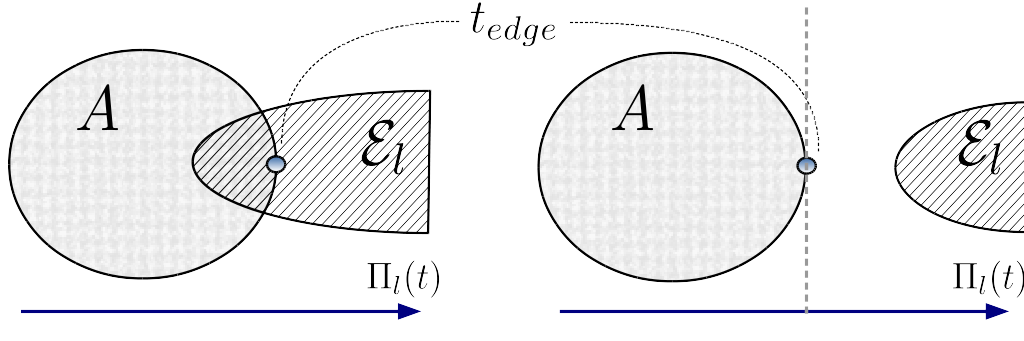
\includegraphics[width=0.85\linewidth]{./pic/algo_sets2}}
\caption{\small Иллюстрация взаимного расположения исследуемых событий и построенного вектора $t_{edge}$ в случае $\P(\Eps_l) > p$ (справа) и в случае $\P(\Eps_l) \leq p$ (слева) для заданного $p \in \zo$.}
\label{ris:algo_sets}
\end{figure}

%$\P(\Eps_l) > p \Leftrightarrow \exists\,{t_{edge}} = (x_{11}, ..., x_{nm}) \in \Eps_l:\; \forall x_{ij}\; \p_{ij}(x_{ij}) > p$, $i \in \{1, ..., n\}$, $j \in \{1, ..., m\}$.



\subsection{Анализ корректности решения $d_*$}
\subsubsection*{Замечание 1}

%Может возникнуть неоднозначность выбора $d_*$, связанная с наличием знаков равенства в цепочке (\ref{e:left_order}). 
Пусть в цепочке (\ref{e:left_order}) $P_* = \P(\Eps_{l_k}) = ... = \P(\Eps_{l_q}) < \P(\Eps_{l_{q+1}})$, $q \geq k$. По построению минимум (\ref{e:zadacha}) достигается на любом решении $d' \subset \Delta \define= \{l_1, ..., l_q\}$, $\abs{d'} = k$, и такое $d'$ сводится к $d_*$ простой заменой индексов. Если $q > k$, следует считать, что решение задачи оптимального выбора объектов не единственное, и сообщить об этом заказчику экспертного опроса. ЛПР может или отказаться от выбора вовсе, например, потребовав дополнительную экспертизу, или выбрать любые $k$ объектов из $\Delta$, или даже отказаться от исходного требования задачи и вместо $k$ выбрать $r$ объектов из $\Delta$, где $k \leq r \leq q$.

\subsubsection*{Замечание 2}
Пусть $E_0 = \{t: \nexists \delta(t)\}$. Это событие возникает, когда найдётся хотя бы $n-k+1$ объектов, для каждого из которых найдётся $k$ объектов не меньшей <<значимости>>:
\begin{equation*}
 E_0 = (\Eps_1 \cap ... \cap \Eps_{n-k+1}) \bigcup (\Eps_2 \cap ... \cap \Eps_{n-k+2}) \bigcup ... \bigcup (\Eps_{k-1} \cap ... \cap \Eps_{n}).
 % надо было бы объедиение по всем возможным наборам, но всё гораздо проще!
\end{equation*}
Событие $E_0$ --- более узкое, чем $\Eps_l$, где требуется $k$ объектов не меньшей <<значимости>> только для объекта $l$:
\begin{equation*}
 E_0 \subset \Eps_l \Rightarrow \Eps_l = E_0 \cup E_l,\;l \in O,
\end{equation*}
где $E_0$ состоит из векторов $t: \nexists \delta(t)$, которые войдут во все $\Eps_l$, а 
$E_l$ --- оставшаяся часть $\Eps_l$. По правилу сложения возможностей:
\begin{equation*}
 \P(\Eps_l) = \sup\{\P(E_0), \P(E_l)\}.
\end{equation*}
%Постоянное первое слагаемое зависит, прежде всего, от выбора $f$ (\ref{e:function_f}). Если оно больше, чем минимум второго слагаемого, для некоторых $l$, возможности таких $\Eps_l$ будут равны, а это может быть плохо для однозначности решения задачи (\ref{e:zadacha}). Поэтому в спорной ситуации, когда в цепочке (\ref{e:left_order}) много равенств, имеет смысл посмотреть на возможность $\P(E_0)$. Если она окажется равна многим $\P(\Eps_l)$, требуется выбрать другую функцию $f$. Если же нет, то спорная ситуация возникла только из-за экспертных $\p_{ij}$.

\section{Оценка, выражающая коллективное мнение группы экспертов}

\section{Примеры использования нашей методики экспертного опроса}
\subsection{Пример 1: Выбор наиболее привлекательных инновационных технологий}

Этот пример построен вокруг проекта, когда наша методика проведения экспертного опроса использовалась крупным инвестором.

Имеется некое множество инновационных технологий $O$. Технология --- результат научно-технической деятельности, который включает в себя изобретения, промышленные образцы, компьютерные программы, технические данные или другие результаты интеллектуальной деятельности и может служить основой определённой практической, в том числе коммерческой деятельности. Каждая технология имеет одного или нескольких правообладателей, получающих выгоду от её применения в практической деятельности. Технологии являются инновационными в том смысле, что обладают значительной новизной и гипотетически имеют большой потенциал для развития, внедрения и получения прибыли, но всё это сопровождается значительным риском. 

Есть крупный инвестор, у которого есть возможность стать совладельцем или полным владельцем технологии, если он вложит деньги и иные ресурсы в её развитие, вступив в сделку с текущими правообладателями. С точки зрения инвестора, технологии обладают разной инвестиционной привлекательностью, которая получается из многих аспектов технологии, среди которых: доходность технологии через год после приобретения, её востребованность на рынке, конкурентоспособность, затраты на внедрение, потенциал интеллектуальной собственности, потенциал кадрового обеспецения, экологические риски, административные риски и т.\,д.

Все аспекты выражаются числами $x_1 \in X_1, x_2 \in X_2, ...$, где мы для простоты положили $X_1 = X_2 = ... = \{0, ..., 10\}$. Инвестиционная привлекательность получается из этих чисел с помощью операций сложения, перемножения и умножения на некоторые коэффициенты в соответствии со специально разработанной блок-схемой (рис.~\ref{ris:tech_scheme}), которая графически выражает функцию $f: x = f(x_1, x_2, ...)$. Каждого эксперта попросили оценить каждую технологию по каждому аспекту. Использовались нечёткие оценки, представленные в виде таблицы <<балл (значение $x \in \{0, ..., 10\}$) --- оценка (значение $p_{\tilde x}(x)$)>>, см.~рис.~\ref{ris:expert_sample}.  

\begin{figure}[H]
\center{\includegraphics[width=0.85\linewidth]{../general_pic/tech_scheme_gold}}
\caption{\small Блок-схема, иллюстрирующая конкретный вид функции $f: x = f(x_1, x_2, ...)$, объединяющей различные аспекты инновационной технологии, оцениваемые экспертом, в итоговую величину инвестиционной привлекательнойсти технологии. }
\label{ris:tech_scheme}
\end{figure}

\begin{figure}[H]
\center{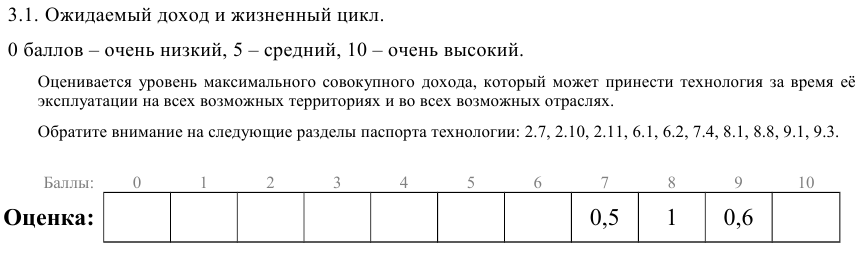
\includegraphics[width=0.85\linewidth]{../general_pic/expert_sample}}
\caption{\small Пример заполненного фрагмента листа экспертого опроса, проведённого по нашей методике. Эксперт выставил нечёткую оценку в ячейках таблицы <<балл (значение $x$) --- оценка (значение $p_{\tilde x}(x)$)>>. Пустым клеткам таблицы соответствуют значения $p_{\tilde x} = 0$. }
\label{ris:expert_sample}
\end{figure}

Интересно отметить, что для различных рисков и других негативных аспектов технологии большие числовые значения интуитивно соотвествуют более плохой ситуации. Это можно учесть либо при составлении функции $f$, либо на других этапах работы. Мы пошли по второму пути (сделали дополнительные указания для экспертов, когда надо <<инвертировать>> оценку), т.\,к. в нашем алгоритме $f$ должна быть монотонной. 

Если делать акцент на команде людей, которые заняты разработкой, практическим применением и/или коммерциализацией инновацонной технологии, то говорят об инновационном проекте или инновацонной компании. Всё, что выше сказано про технологии, остаётся верно и для компаний; разница только в том, что некоторые инвесторы обладают собственным кадровым обеспечением и предпочитают трансфер готовых технологий, в то время как другие делают ставку на потенциал команды инновационной компании.

\subsection{Пример 2: Выбор наиболее точного измерительного прибора}

Выбор измерительного прибора мы будем рассматривать в контексте теории измерительно-вычислительнх преобразователей как средств измерений (ИВП) Ю.~П.~Пытьева \cite{4}.

%для диплома
%T состоит из векторов t, а Омега из событий вида {тета=t}, но у них одинаковая размерность

%контрольный вектор -- на границе события {Ek > p}





\section{Заключение}



% Список литературы


\end{document}